\documentclass{article}

%\usepackage[math,lf,footnotefigures]{MyriadPro}
%\renewcommand{\familydefault}{\sfdefault}
%\usepackage[T1]{fontenc}

\usepackage{tikz}
\usetikzlibrary{arrows}
\usetikzlibrary{arrows.meta}
\usetikzlibrary{positioning}

\usepackage{xcolor}
\definecolor{ufzgray1}{RGB}{126,126,126}
\definecolor{ufzgray2}{RGB}{156,156,156}
\definecolor{ufzgray3}{RGB}{185,185,185}
\definecolor{ufzgray4}{RGB}{230,230,230}

% adjust the page margins
\usepackage[left=2.7cm,right=2.5cm,top=1.2cm,bottom=1cm]{geometry}

\begin{document}
	
\pagestyle{empty}

\hspace*{-3cm}
	\begin{tikzpicture}[scale=2.5]
		\tikzstyle{block} = [rectangle, draw, fill=white!20, 
		text width=7em, text centered, rounded corners, minimum height=1em]
		\tikzstyle{blockwide} = [rectangle, draw, fill=white!20, 
		text width=14.5em, text centered, rounded corners, minimum height=1em]
		\tikzstyle{noblock} = [rectangle, %fill=white!20, 
		text width=7.0em, rounded corners, minimum height=1em]
		\tikzstyle{noblockwide} = [rectangle, %fill=white!20, 
		text width=16.0em, rounded corners, minimum height=1em]
		\tikzstyle{abcblock} = [rectangle, fill=white!20, 
		text width=1em, rounded corners, minimum height=1em]
		\tikzstyle{line} = [draw, -latex']
		\tikzstyle{line} = [draw,latex'-latex'new]
		
		%
		\draw[black,rounded corners,fill=ufzgray1!5] (-0.7,0.65) -- (6.8,0.65) -- (6.8,-1.15) -- (-0.7,-1.15) --cycle;
		
		%
		\draw[black,rounded corners,fill=ufzgray1!5] (-0.7,-1.25) -- (6.8,-1.25) -- (6.8,-3.05) -- (-0.7,-3.05) --cycle;
		
		%
		\draw[black,rounded corners,fill=ufzgray1!5] (-0.7,-3.15) -- (6.8,-3.15) -- (6.8,-4.95) -- (-0.7,-4.95) --cycle;
		
		%
		\draw[black,rounded corners,fill=ufzgray1!5] (-0.7,-5.05) -- (6.8,-5.05) -- (6.8,-8.75) -- (-0.7,-8.75) --cycle;
		
		\node (figa) at (0.0,0) {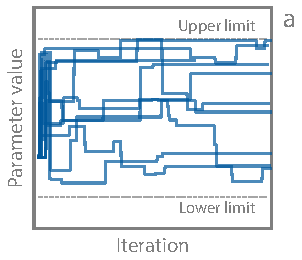
\includegraphics[width=3cm]{figure_11-01.pdf}};
		\node (figb) at (2.5,0) {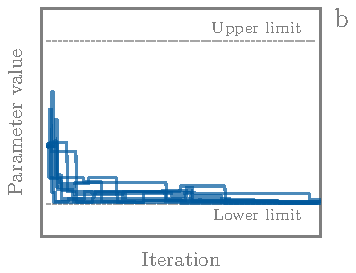
\includegraphics[width=3cm]{figure_11-02.pdf}};
		\node (figc) at (5.0,0) {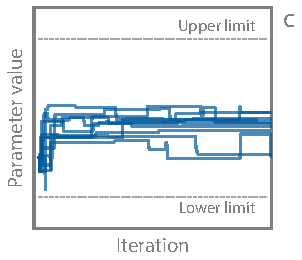
\includegraphics[width=3cm]{figure_11-03.pdf}};
		
		\node (figd) at (0.0,-1.9) {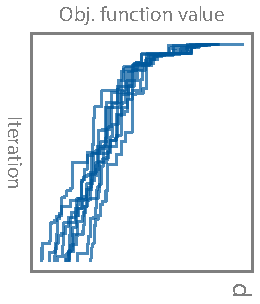
\includegraphics[height=3cm,angle=90]{figure_11-04.pdf}};
		\node (fige) at (2.5,-1.9) {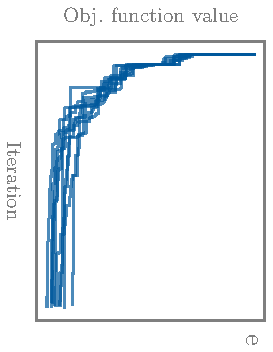
\includegraphics[height=3cm,angle=90]{figure_11-05.pdf}};
		\node (figf) at (5.0,-1.9) {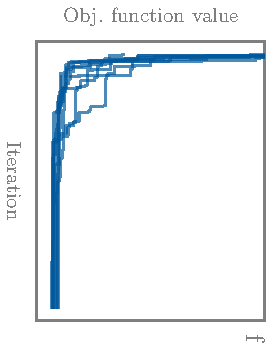
\includegraphics[height=3cm,angle=90]{figure_11-06.pdf}};
		
		\node (figg) at (0.0,-3.8) {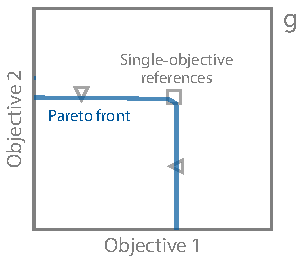
\includegraphics[width=3cm]{figure_11-07.pdf}};
		\node (figh) at (2.5,-3.8) {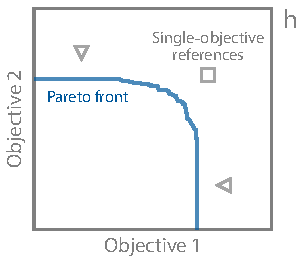
\includegraphics[width=3cm]{figure_11-08.pdf}};
		\node (figi) at (5.0,-3.8) {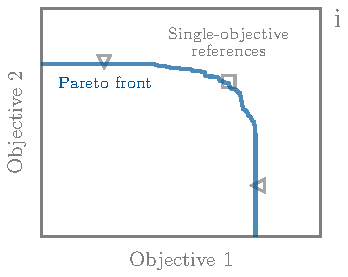
\includegraphics[width=3cm]{figure_11-09.pdf}};
		
		\node (figj) at (0.0,-5.7) {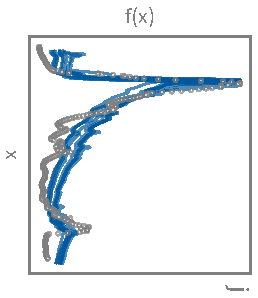
\includegraphics[height=3cm,angle=90]{figure_11-10.pdf}};
		\node (figk) at (2.5,-5.7) {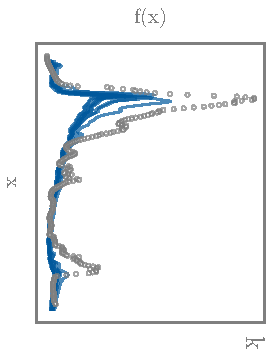
\includegraphics[height=3cm,angle=90]{figure_11-11.pdf}};
		\node (figl) at (5.0,-5.7) {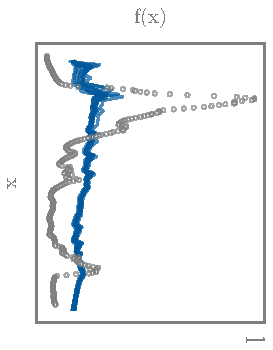
\includegraphics[height=3cm,angle=90]{figure_11-12.pdf}};
		
		\node (figm) at (0.0,-7.6) {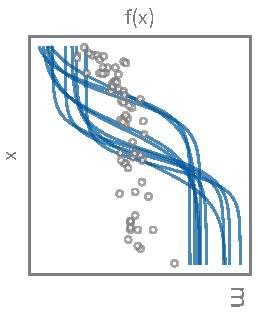
\includegraphics[height=3cm,angle=90]{figure_11-13.pdf}};
		\node (fign) at (2.5,-7.6) {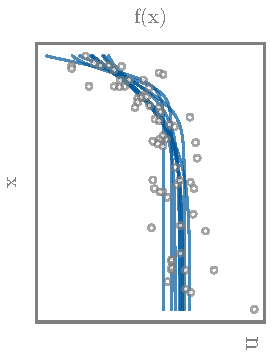
\includegraphics[height=3cm,angle=90]{figure_11-14.pdf}};
		\node (figo) at (5.0,-7.6) {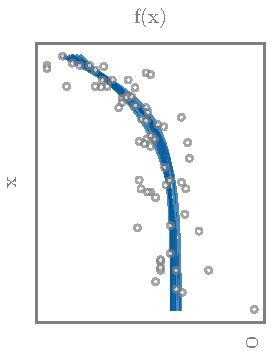
\includegraphics[height=3cm,angle=90]{figure_11-15.pdf}};
		
		% left side "captions"
		\node [align=center,left of=figa, rotate=90,yshift=1.5cm,xshift=-0.6cm] {{\large Check}\\[3pt]{\large Parameter values}};
		\node [align=center,left of=figd, rotate=90,yshift=1.72cm,xshift=-0.6cm] {{\large Check}\\[3pt]{\large Obj. function values}\\[3pt]{\large --~Single-objective~--}};
		\node [align=center,left of=figg, rotate=90,yshift=1.72cm,xshift=-0.6cm] {{\large Check}\\[3pt]{\large Obj. function values}\\[3pt]{\large --~Multi-objective~--}};
		\node [align=center,left of=figj, rotate=90,yshift=1.5cm,xshift=-2.5cm,xshift=-0.6cm] {{\large Check}\\[3pt]{\large Fit of simulations and observations}};
		
		% right side reference to sections
		\node [align=center,left of=figa, rotate=90,yshift=-18.3cm,xshift=-0.6cm,color=ufzgray1] {[used in Sect.~2.6]};
		\node [align=center,left of=figd, rotate=90,yshift=-18.3cm,xshift=-0.6cm,color=ufzgray1] {[used in Sect.~2.8]};
		\node [align=center,left of=figg, rotate=90,yshift=-18.3cm,xshift=-0.6cm,color=ufzgray1] {[used in Sect.~2.9]};
		\node [align=center,left of=figj, rotate=90,yshift=-18.3cm,xshift=-0.6cm,color=ufzgray1] {[used in Sect.~2.7]};
		\node [align=center,left of=figm, rotate=90,yshift=-18.3cm,xshift=-0.6cm,color=ufzgray1] {[used in Sect.~2.6]};
		
		% what's wrong :: A-C
		\node [noblock,align=left,left of=figa,xshift=3.8cm] {{\scriptsize \underline{Problem}}\\no consistent final value; spread entire range};
		\node [noblock,align=left,left of=figb,xshift=3.8cm] {{\scriptsize \underline{Problem}}\\converges but against limit of parameter range};
		\node [noblock,align=left,left of=figc,xshift=3.8cm] {{\scriptsize \underline{No Problem}}\\all trials consistent; converge within parameter range};
		
		% what to do :: A-C
		\node [noblockwide,align=left,below of=figa,yshift=-1.1cm,xshift=1.4cm] {\textit{parameter might be insensitive/not inferable with given data; consider sensitivity analysis to check}};
		\node [noblockwide,align=left,below of=figb,yshift=-1.1cm,xshift=1.4cm] {\textit{parameter range (here lower limit) might be too restricted; consider widening range}};
		\node [noblockwide,align=left,below of=figc,yshift=-1.1cm,xshift=1.4cm] {\textit{success}};
		
		% what's wrong :: D-F
		\node [noblock,align=left,left of=figd,xshift=3.8cm,text width=7.5em] {{\scriptsize \underline{Problem}}\\downward trend of each trial; no plateau};
		\node [noblock,align=left,left of=fige,xshift=3.8cm] {{\scriptsize \underline{Problem}}\\trials converge but not to consistent value};
		\node [noblock,align=left,left of=figf,xshift=3.8cm,text width=7.5em] {{\scriptsize \underline{No Problem}}\\all trials plateau; converge to similar values};
		
		% what to do :: D-F
		\node [noblockwide,align=left,below of=figd,yshift=-1.1cm,xshift=1.4cm] {\textit{convergence criterion or budget used likely not appropriate; consider adjusting}};
		\node [noblockwide,align=left,below of=fige,yshift=-1.1cm,xshift=1.4cm] {\textit{increase budget or try another calibration algorithm; parameter ranges might be too wide}};
		\node [noblockwide,align=left,below of=figf,yshift=-1.1cm,xshift=1.4cm] {\textit{success}};
		
		% what's wrong :: G-I
		\node [noblock,align=left,left of=figg,xshift=3.8cm] {{\scriptsize \underline{Problem}}\\degenerated front (only visible when magnifying)};
		\node [noblock,align=left,left of=figh,xshift=3.8cm] {{\scriptsize \underline{Problem}}\\front not consistent with single-objective references};
		\node [noblock,align=left,left of=figi,xshift=3.8cm,text width=7.5em] {{\scriptsize \underline{No Problem}}\\front visible and consistent with single-objective references};
		
		% what to do :: G-I
		\node [noblockwide,align=left,below of=figg,yshift=-1.1cm,xshift=1.4cm] {\textit{objectives are not independent; consider using only subset of objective functions}};
		\node [noblockwide,align=left,below of=figh,yshift=-1.1cm,xshift=1.4cm] {\textit{results not converged yet; increase budget or try another calibration algorithm}};
		\node [noblockwide,align=left,below of=figi,yshift=-1.1cm,xshift=1.4cm] {\textit{success}};
		
		% what's wrong :: J-L
		\node [noblock,align=left,left of=figj,xshift=3.8cm] {{\scriptsize \underline{Problem?}}\\fit favors high observation\\values};
		\node [noblock,align=left,left of=figk,xshift=3.8cm] {{\scriptsize \underline{Problem?}}\\fit favors low observation\\values};
		\node [noblock,align=left,left of=figl,xshift=3.8cm] {{\scriptsize \underline{Problem?}}\\fit focuses\\on average\\behavior};
		
		% what to do :: J-L
		\node [noblockwide,align=left,below of=figj,yshift=-1.1cm,xshift=1.4cm] {\textit{if this not desired, consider replacing, e.g., MSE with mean absolute error (MAE), or log-transform data}};
		\node [noblockwide,align=left,below of=figk,yshift=-1.1cm,xshift=1.4cm] {\textit{if this is not desired, consider higher weights for large y-values and errors (e.g., use MSE, not MAE)}};
		\node [noblockwide,align=left,below of=figl,yshift=-1.1cm,xshift=1.4cm] {\textit{if this is not desired, consider weights for y-values or change objective function entirely}};
		
		% what's wrong :: M-O
		\node [noblock,align=left,left of=figm,xshift=3.8cm] {{\scriptsize \underline{Problem}}\\generally poor fit; wide spread of trials};
		\node [noblock,align=left,left of=fign,xshift=3.8cm] {{\scriptsize \underline{Problem}}\\fit follows trend of data; wide spread of trials};
		\node [noblock,align=left,left of=figo,xshift=3.8cm] {{\scriptsize \underline{No Problem}}\\fit follows trend of data; narrow spread of trials};
		
		% what to do :: M-O
		\node [noblockwide,align=left,below of=figm,yshift=-1.1cm,xshift=1.4cm] {\textit{parameter ranges might be too narrow; potentially consider revising model if ranges already wide}};
		\node [noblockwide,align=left,below of=fign,yshift=-1.1cm,xshift=1.4cm] {\textit{parameter ranges too wide or budget for calibration too low; consider revising}};
		\node [noblockwide,align=left,below of=figo,yshift=-1.1cm,xshift=1.4cm] {\textit{success}};
		
	\end{tikzpicture}

\end{document}



